\begin{figure}
      \begin{subfigure}{1.0\textwidth}
  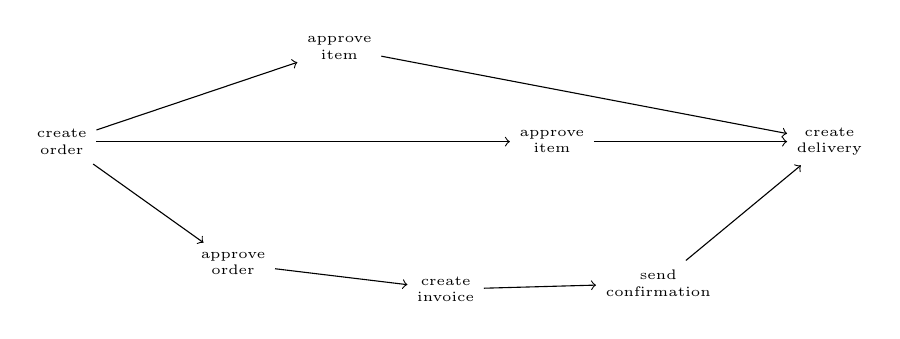
\begin{tikzpicture}
      \draw[align=center,font=\tiny]
        (-10.2, 3.019) node (0){create\\order}
        (-8.025, 1.469) node (1){approve\\order}
        (-3.975, 3.019) node (2){approve\\item}
        (-6.675, 4.206) node (3){approve\\item}
        (-5.325, 1.144) node (4){create\\invoice}
        (-2.625, 1.219) node (5){send\\confirmation}
        (-0.45, 3.019) node (6){create\\delivery};
      \begin{scope}[->]
        \draw (0) to (1);
        \draw (0) to (2);
        \draw (0) to (3);
        \draw (1) to (4);
        \draw (2) to (6);
        \draw (3) to (6);
        \draw (4) to (5);
        \draw (5) to (6);
      \end{scope}
    \end{tikzpicture}

  \end{subfigure}
  \begin{subfigure}{1.0\textwidth}
  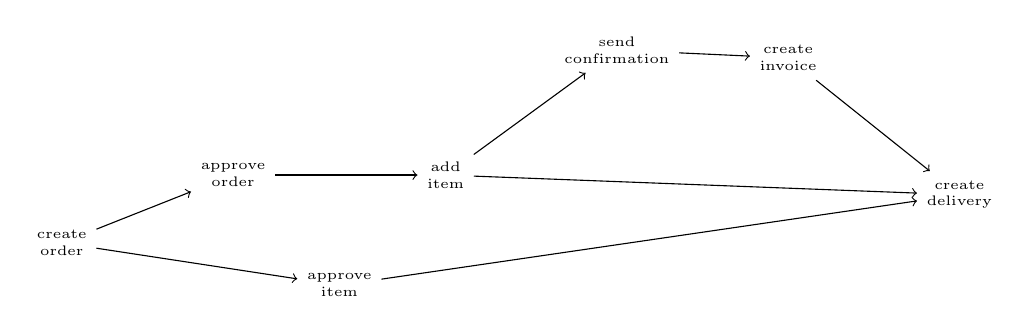
\begin{tikzpicture}
      \draw[align=center,font=\tiny]
        (-11.85, 1.464) node (7){create\\order}
        (-8.325, 0.926) node (8){approve\\item}
        (-9.675, 2.326) node (9){approve\\order}
        (-6.975, 2.326) node (10){add\\item}
        (-4.8, 3.914) node (11){send\\confirmation}
        (-2.625, 3.814) node (12){create\\invoice}
        (-0.45, 2.076) node (13){create\\delivery};
      \begin{scope}[->]
        \draw (7) to (8);
        \draw (7) to (9);
        \draw (8) to (13);
        \draw (9) to (10);
        \draw (10) to (11);
        \draw (10) to (13);
        \draw (11) to (12);
        \draw (12) to (13);
      \end{scope}
    \end{tikzpicture}

  \end{subfigure}
    
  \caption{Process executions}
    \label{fig:process-executions}
\end{figure}
